\documentclass[xcolor={usenames,dvipsnames,svgnames}]{beamer}

\usetheme{mun}
\setbeamercovered{transparent}
\usepackage{multido}

\usepackage{biblatex}
\bibliography{\jobname}

\setbeamertemplate{itemize item}{\scriptsize\raise1.25pt\hbox{\donotcoloroutermaths$\blacktriangleright$}}
\setbeamertemplate{itemize subitem}{\tiny\raise1.5pt\hbox{\donotcoloroutermaths$\blacktriangleright$}}
\setbeamertemplate{itemize subsubitem}{\tiny\raise1.5pt\hbox{\donotcoloroutermaths$\blacktriangleright$}}

\title{Text Summarization}
\subtitle{Computer Science 4750}
\author{Noah~Gallant\,~//~Jacob~House}
\date{Fall 2018}

\begin{document}
\begin{frame}[plain]
\titlepage
\end{frame}

\startheads

\section{Topic}
\begin{frame}

{\large\bfseries Text Summarization // Automatic Abstracting}
\vskip 6pt
The process of reducing an input text to a smaller, more concise version of itself.
\vskip 6pt
Use cases include: search engine results, academic research, legal contract analysis, and more advanced email inbox filtering.
\vfill

\end{frame}

\section{Different Approaches}

\subsection{Evolutionary Algorithm}
\begin{frame}
%Different candidate summarizations are made and a score each of their fitnesses is computed. Those with the highest fitness move on to create new offspring candidates which share positive traits of both parents.
\begin{tabular}{ll}
	\begin{minipage}{0.6\linewidth}
		\begin{enumerate}
			\item Assign weights to text features
			\item Create population of distinct summaries
			\item Assess fitness
			\item Choose summaries with highest fitness
			\item Create offspring from chosen summaries
			\item Repeat steps 3--5 until the summary is concise enough
		\end{enumerate}
	\end{minipage}
	& \begin{tabular}{c}
		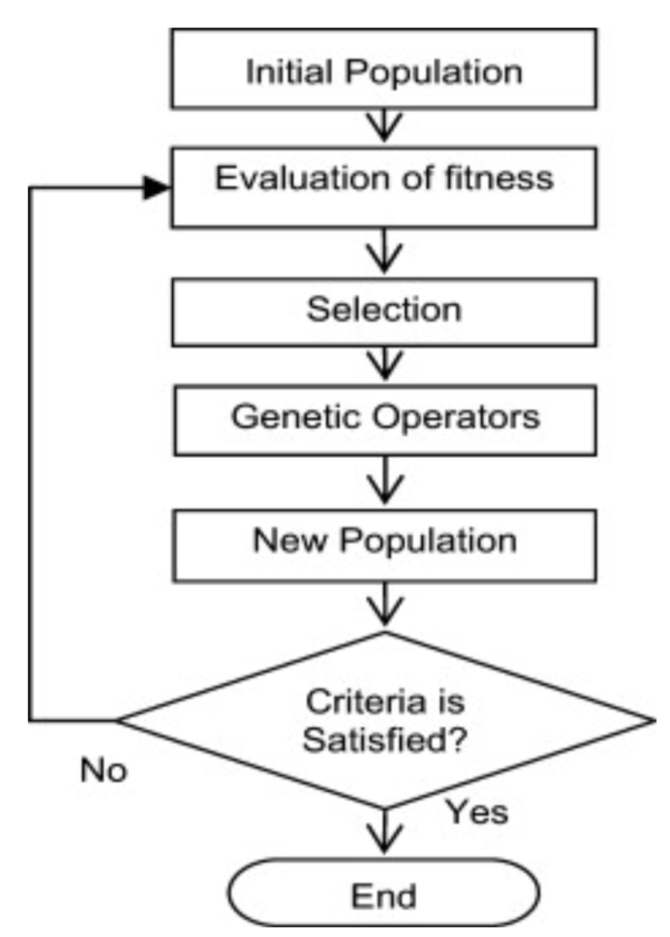
\includegraphics[width=0.3\linewidth]{ga}
	\end{tabular}
\end{tabular}
\end{frame}

\subsection{Nested Tree}
\begin{frame}
The goal in this approach is to repeatedly trim the tree until the desired summary size is reached.
\vskip 1pc
\begin{tabular}{ll}
\begin{minipage}{0.45\linewidth}
\begin{itemize}
	\item Tree structure is dependency based
	\begin{itemize}
		\item Inter-sentence
		\item Inter-word
	\end{itemize}
	\vskip 1pc
	\item Tree trimming to reduce size
	\begin{itemize}
		\item Removes duplicates
		\item Removes less important nodes
	\end{itemize}
\end{itemize}
\end{minipage}
& \begin{tabular}{c}
	\hskip -3pc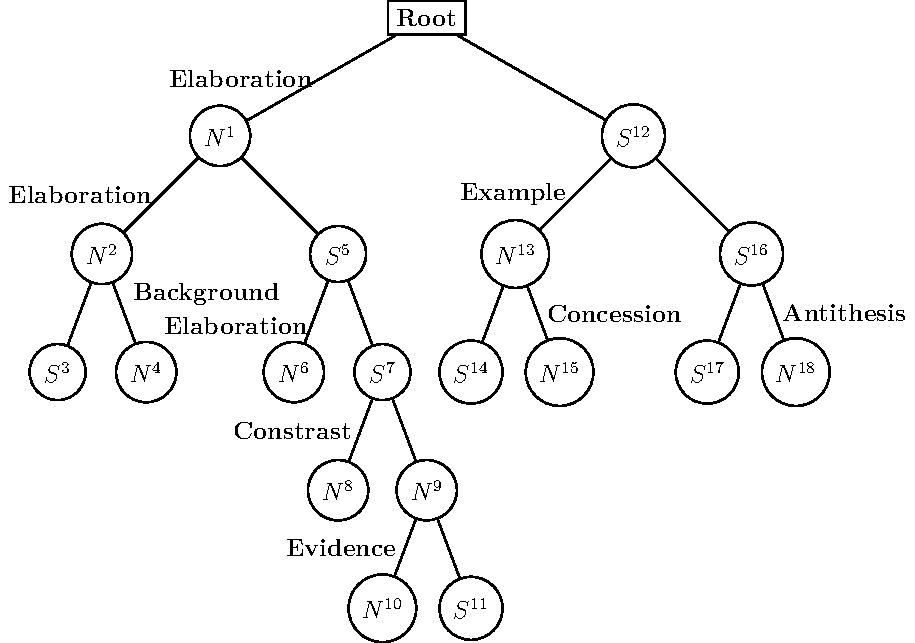
\includegraphics[width=0.6\linewidth]{tree}
\end{tabular}
\end{tabular}
\end{frame}

\subsection{Graph-Based}
\begin{frame}
\begin{itemize}
	\item Nodes created for each sentence
	\vskip 6pt
	\item Edges added between sentence nodes
	\vskip 0pt
	\begin{itemize}
		\item Adjacent sentences in the text
		\vskip 4pt
		\item Sentences that share common words
		\vskip 6pt
	\end{itemize}
	\item Edges with higher weight denote dependency
	\vskip 6pt
	\item Nodes (sentences) with highest total edge weight should be included in the summary
\end{itemize}
\end{frame}

\section{Our Design}
\multido{\i=1+1}{4}{%
\begin{frame}
	\centering
	\includegraphics[width=.75\linewidth]{venn-\i}
\end{frame}
}

\section{Implementation}
\subsection{Preprocessing}
\begin{frame}
\begin{itemize}
	\item Sentence separation
	\item Deals with special/unicode characters
\end{itemize}
\end{frame}
\subsection{The {\tt Graph} Class}
\begin{frame}
The {\tt Graph} class is a singleton which contains all the nodes and edges. It is the responsibility of this class to do the text preprocessing, and to create nodes and the edges between them.
\begin{itemize}
	\item Contains a list of:
	\begin{itemize}
		\item Nodes
		\item Edges
		\item Words in the text
	\end{itemize}
\end{itemize}
\end{frame}
\subsection{The {\tt Node} Class}
\begin{frame}
A new node object is created for every sentence in the input text. It contains the sentence, a list of words in the sentence, and a list of edges which associate it with other sentence nodes.
\begin{itemize}
	\item Initialized with 2 edges
	\begin{enumerate}
		\item Connecting the preceding sentence
		\item Connecting the following sentence
	\end{enumerate}
	\item More edges are added between nodes that share a common word
\end{itemize}
\end{frame}
\subsection{The {\tt Edge} Class}
\begin{frame}
The {\tt Edge} class contains the two nodes it is connecting, as well as the information about the connection.
\vskip 1pc
This information includes the words connecting the sentences, as well as if they are sentences connected by proximity.
\end{frame}

\nohead
\section{Questions?}
\begin{frame}

{\huge\bfseries Questions?}
\end{frame}

\section{References}
\begin{frame}[allowframebreaks]
\nocite{*}
\printbibliography
\end{frame}
\end{document}